\chapter{Data Preparation}
    Data preparation is the process of transforming the acquired dataset into a dataset which can be fed into learning algorithms and is cleaned of impurities in such a way, that the learning results are likely satisfactory. Impurities to some extent were already identified in the prior chapter, additionally, shifted columns, encoding errors or different data formats have to be accounted for.
	Data preparation includes data wrangling, data cleaning, and feature extraction. What is left should be a uniform dataset, which is in a format that is understandable by the desired algorithms.
	
	\section{Data processing and data wrangling}

        \subsection{Alternatives}
        The chosen dataset consists of files in \ac{JSON} format. Several alternatives for storage and transforming the data exist. 
        
        \paragraph{Storage Location}
        Within the constraints of the thesis, three options are available for data storage. Firstly, data can be stored locally on the available machine. The data is available without internet access, and the local machine has high read/write speeds. This option requires no additional learning, and is free of charge for the department. A multitude of libraries exist for accessing files on a local file system. A downside is the limited scalability in terms of storage capacity and read/write operations. Additionally, local storage makes the data only available to this specific machine.
        
        Storing data on a cloud file sharing system is easy to operate and free of usage-bound charges. The storage space is virtually unlimited. Accessing files on sharing platforms is feasible but tedious. The access can be shared within the company context, but everyone is subject to the limited accessibility. Using a files storage service could be of use for transferring data without a physical connection. Still, this is the only recommended use case in this context.
        
        The third option is storing the data using a specialized storage service, such as AWS S3. While the learning overhead is higher in the beginning, the scalability is a convincing argument. Billing is according to usage, but adequate because of the high connectivity with other cloud-based ML service offerings inside and outside of SAP.
        
        \begin{table}[ht]
            \centering
            \caption{Comparison of available Storage Options}
            \begin{tabular}{clll}
                \toprule
                &\textbf{Local} & \textbf{Cloud Filesharing} & \textbf{Specialized Storage Services} \\
                \midrule
                
                Example     & \begin{tabular}[c]{@{}l@{}}2.6GHz \\ 512GB SSD\end{tabular} & Microsoft OneDrive                                                        & AWS S3                                                                                                 \\
                \midrule
                Ease of use & high                                                        & high                                                                      & higher learning overhead                                                                               \\
                \midrule
                Cost        & free of charge                                              & free of charge                                                            & \begin{tabular}[c]{@{}l@{}}billing according to \\ used storage space\end{tabular}                     \\
                \midrule
                Scalability & limited                                                     & unlimited                                                                 & unlimited                                                                                              \\
                \midrule
                Data access & local                                                       & \begin{tabular}[c]{@{}l@{}}limited remote \\ access capacity\end{tabular} & \begin{tabular}[c]{@{}l@{}}local, remote, high \\ connectivity to \\ ML service offerings\end{tabular}\\
				\bottomrule
                
            \end{tabular}
            \label{tabelle:storage}
        \end{table}
        
        \paragraph{Data Format}
        The data is still available only in the from \ac{JSON} documents. Python allows for easy parsing of these objects, but this option is highly inefficient compared to native Python data structures.
        The equivalent to \ac{JSON} in Python are combinations between lists and dictionaries. Dictionaries are an implementation of the \lstinline|Map| data structure.
        
        This option stands in contrast to a data format commonly used in data science tasks: the \lstinline|DataFrame|. Both formats, the dictionaries and DataFrames have specific advantages and disadvantages.
        
        The \lstinline|DataFrame| is structured like a table, consisting of labeled rows and columns. This data structure is implemented in the library \lstinline|pandas|. 
        Different data formats such as strings, floats or boolean values can be stored in the table.        Optimized methods for calculating row-wise and column-wise operations are supplied in the library. This makes the \lstinline|DataFrame| one of the most popular tools for data scientists.
        
       \lstinline|DataFrame|s being suited for various purposes, makes them inflated and slower than low-level data structures. The indexing operation, for example, has to address a multitude of cases. This makes it slower than a simple dictionary access. Appendix \ref{benchmarkDF} details the comparison in a benchmark.
       
       Surprisingly, storing \ac{JSON} data in a \lstinline|DataFrame| is less memory-intensive than storing the same data in dictionaries and lists \cite{DFvsJSON}. This means  \lstinline|DataFrame|s are favorable for storage and calculations with large data quantities.
       
       Considering all factors, the best choice is transforming the dataset into a  \lstinline|DataFrame|. Still, the advantages of dictionaries and lists in basic use-cases will be kept in mind for later.
     
    \subsection{Theoretical Implementation}
    For the data wrangling the invoices have to be read into memory and then processed into a reusable structure. All invoices will be combined into \lstinline|DataFrame|s, which then are persisted for later use.
	
    \begin{figure}[ht]
        \centering
        \includegraphics[height=5cm]{Bilder/practical/entity_relationship.png}
        \caption{Entity Relationship Diagram for Invoice Documents}
        \label{fig:er}
    \end{figure}
	The documents can be separated into two fundamental entities: the invoice and the line items. The entity relationship diagram (\ref{fig:er}) shows how invoices and line items are related. The invoice contains at least one line item, and the information in the invoice is relevant to all of its line items. This includes information about the vendor, and the invoice date. The line items of an invoice contain specific information on the products, such as the material number and the description.
	An invoice and its line items can be matched through an unique identifier, which is also the filename.

	 \begin{figure}[ht]
		\centering
		\includegraphics[height=11.5cm]{Bilder/preprocessing/df_schema.png}
		\caption{Theoretical Implementation of the Data Wrangling}
		\label{fig:invoice_df_schema}
	\end{figure}	

	Now, looking at the technical side of the file composition.	The data for an invoice and its line items is stored in an array of objects. The array "annotations" contains objects, each one representing information such as the invoice date or the unit price. A schematic description of how the invoice data should be represented after extraction is shown in Figure \ref{fig:invoice_df_schema}: One invoice is modeled as one row in the table. Different attributes are represented as columns.
	Information about line items have labels containing the prefix "lineItem". One invoice containing several items is represented by duplicate values of one label (in the example \ref{fig:invoice_df_schema} the label "lineItem.description.value"). Each new label "lineItem.description.value" denotes a new line item. Here, the order of the labels has to be retained during data wrangling to ensure not mixing up information about different invoice items. Each new line item should be a new row in the table of line items.
	
	The goal of the data wrangling process is to create two \lstinline|DataFrame|s, one for the invoices and one for the line items.
	Additionally, another data structure will be created to optimize recurring and complex operations.
	
	Data exploration shows, there are only 79.741 unique descriptions for the listed items. By saving only the unique values, the required space is reduced to less than one fourth compared to before. Additionally, this step is required by most machine learning models, as duplicate input values can skew the outcome. The model is chosen later, so this processing step leaves the model selection more open to different kinds of learning algorithms.
	
	After the deletion of duplicate descriptions, the relationship between one line item and its description is not one-to-one, but rather one description belonging to several different line items. Model outputs will be a classification of one description, so to restore the relationship between the classification result and one line item, a mapping is constructed.
	This dictionary maps one description to all line items (more specifically, their ID) with this description.
	\begin{figure}[ht]
		\centering
		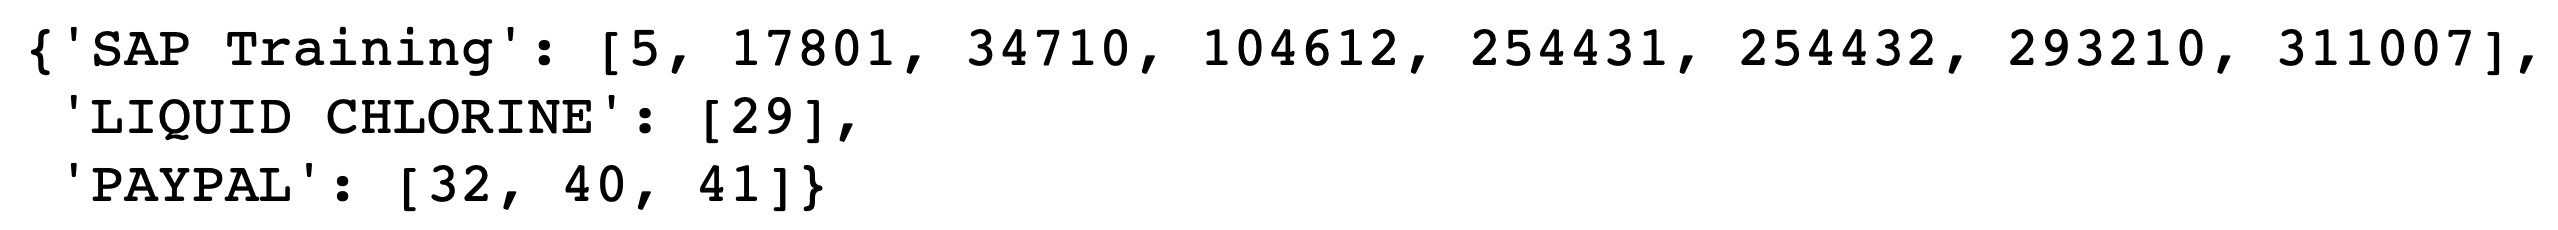
\includegraphics[width=\linewidth]{Bilder/description_map.png}
		\caption{Mapping Descriptions to their Line Item IDs}
		\label{fig:mapping}
	\end{figure}


	After the construction of both tables and the mapping, these artifacts should be serialized. This way, they can easily be loaded into memory without the effort to reconstruct them from scratch.
	
    \subsection{Practical Implementation}
	
	The files were processed using a Python script (\ref{code:InvoiceReader}). The information on invoices is stored in a tabular data structure, a \lstinline|pandas DataFrame|. Worth mentioning is that some invoices contain more information than others. In this case, invoices are still appended into one table, but fields for non-existent values are left empty. In Figure \ref{fig:df-invoices}, the first invoice does not have a total amount included, but since the second one does, this column is created.
	The filename of one invoice contains the unique identifier for one invoice.
	
	\begin{figure}[ht]
		\centering
		\includegraphics[height=2.5cm]{Bilder/practical/df_invoices.png}
		\caption{Exemplary depiction for processed invoices in a DataFrame}
		\label{fig:df-invoices}
	\end{figure}

	Similarly, information on the invoice items is retrieved from the documents and stored in a \lstinline|pandas DataFrame|. Every line item has an unique id and can also be linked to the respective invoice through the filename.
	
	\begin{figure}[ht]
		\centering
		\includegraphics[height=6cm]{Bilder/practical/df_lineitems.png}
		\caption{Exemplary depiction for processed invoice items in a DataFrame}
		\label{fig:df-invoice}
	\end{figure}
	
	The resulting two \lstinline|DataFrame|s are serialized with the Python standard library \lstinline|pickle|. The data can be efficiently loaded into memory and re-serialized again with this library.
	
	This processing step allowed for storing the initial 5.12GB of data in a more usable format and takes up only a total of 393MB.

	The process of reading files from the disk is not inherently an expensive one, but in the realms of many thousand documents, processing times soon reach several days. Observing the execution of the Python code showed a peculiarity: While the utilization of the used processor was consequently at the maximum (in Figure \ref{fig:cpu} at 97.1\%), only one process is executed, leaving the total \ac{CPU} usage at only 20\%. 
	
	\begin{figure}[ht]
		\centering
		\includegraphics[height=5cm]{Bilder/practical/python_processes.png}
		\caption{\acs{CPU} Usage during single-process Python Execution}
		\label{fig:cpu}
	\end{figure}
	
	
	One question that may now arise is: Why doesn't Python split up the workload and employ the full capacity of the machine?
	This can be explained with the design of the Python interpreter. The Global Interpreter Lock controls access to the Python Virtual Machine executing the code. This lock only allows exactly one thread to run at a time \cite[ch.~18.3.1]{corePython}. This of course is not favorable, as valuable CPU capacity is idle. Fortunately, the lock behaves in a special way regarding C routines: the lock is released before executing C code \cite[ch.~18.3.1]{corePython}. I/O operations in Python, such as opening files, utilize C code. This allows to bypass the, in this case, inconvenient locking mechanism. 
	
	Different Python libraries exploit this specialty and allow to spawn a pool of different processes, which then execute calls asynchronously. The \lstinline|ProcessPoolExecutor| is one example of multiprocessing.
	
\begin{lstlisting}[language=python, 
label=code:process-pool,
caption=Spawning a Process Pool in Python,
style=EigenerPythonStyle]   
with concurrent.futures.ProcessPoolExecutor() as executor:
	results = process_map(r.read_invoice, filenames, chunksize=2000)
\end{lstlisting}

	The \lstinline|ProcessPoolExecutor| (s. listing \ref{code:process-pool}) can distribute a list of input values for functions (\lstinline|filenames| ) onto a function (\lstinline|r.read_invoice|). Additionally, the \lstinline|chunksize| as parameter specifies how large the bundles of input values for each process are. Distributing the workload onto all \ac{CPU} cores, the processing time was reduced from 27 hours to under 4 minutes. 
	
	\section{Data cleaning}
	Data cleaning concerns removing all impurities from the data. This includes deleting duplicates, using an uniform data type, and removing unnecessary information.
	Just the descriptions of all the line items will be fed into models, therefore only those have to be cleaned. The Python library \ac{NLTK} provides useful methods for cleaning textual data.
	
	\lstinputlisting[
	label=code:cleaner,    % Label; genutzt für Referenzen auf dieses Code-Beispiel
	caption=Python Script for extracting JSON Data into a DataFrame,
	captionpos=b,               % Position, an der die Caption angezeigt wird t(op) oder b(ottom)
	style=EigenerPythonStyle,   % Eigener Style der vor dem Dokument festgelegt wurde
	firstline=0,                % Zeilennummer im Dokument welche als erste angezeigt wird
	lastline=23                 % Letzte Zeile welche ins LaTeX Dokument übernommen wird
	]{Quellcode/cleaner}
	
	In the code example \ref{code:cleaner}, the text is firstly separated into tokens. Then each token is examined whether it contains non-alphabetic characters. Only alphabetic tokens are retained. Again, this process is highly computationally intensive due to the size of the data. Therefore, this task was completed using the same procedure for multiprocessing as detailed in the prior section.
	
\begin{lstlisting}[
	language=sh,
	caption=A Description before and after Data Cleaning,
	label=code:cleaned_descr
	]
$ python3 -c 'import cleaner; print(cleaner.clean("500grams of special baking flour type 504"))' \\
>>>  ['of', 'special', 'baking', 'flour', 'type']
\end{lstlisting}
	 
	 The code example \ref{code:cleaned_descr} shows the input and output of this procedure. A token is completely discarded if it contains non-alphabetical characters, as these tokens are more than often not an accurate descriptor of the text's meaning.	

        
        \section{Feature Extraction and Feature Engineering}
        \label{section:feature-extraction}
        The majority of popular \ac{ML} algorithms require the input of scalar, vector or matrix data. Several methods for representing text as mathematical object will be discussed in the following.
    
            \subsection{Alternatives}
            Firstly, the distributional representations will be explained and evaluated.
            
            \subsubsection{Term-Document Incidence Matrix}
			\label{section:tdim}
            \begin{figure}[h]
            	\centering
            	 \includegraphics[height=3.5cm]{Bilder/corpus_bow.png}
            	\caption{Example Corpus}
            	\label{fig:term-doc-incidence}
            \end{figure}
            The three documents in Figure \ref{fig:corpus} will be considered to explain the workings of the one-hot encoding. A corpus is transformed into a term-document incidence matrix representation in two steps. 
            
            \begin{figure}[h!]
            	\centering
            	\includegraphics[height=2.5cm]{Bilder/preprocessing/term-document-incidence.png}
            	\caption{Term-Document Incidence Matrix}
            	\label{fig:corpus}
            \end{figure}
            
            Firstly, the vocabulary is determined. 
            It is a collection of all words occurring in the corpus. Every word is contained exactly once, regardless of the actual number of occurrences. The vector representation of one document is of the same length as the vocabulary. One document being represented by one vector, a corpus of several documents can be represented as a matrix. The resulting matrix $M$ has the size $ |D|*|V| $, with $|D|$ being the number of documents in the corpus, and $|V|$ being the size of the vocabulary.
            
            Secondly, for each combination of one document $ d_{i} $ and one word $ v_{j} $ in the vocabulary, it is determined whether the word occurs in the document. This information is encoded binary with a "1" at $m_{ij}$ for occurrence and a "0" for no occurrence. The resulting vectors for the three documents are:
            \[ d_{1} = [0,1,0,0,0,1,0,0] \]
            \[ d_{2} = [1,0,1,0,1,0,1,1] \]
            \[ d_{3} = [0,0,0,1,0,0,0,1]\]
    		The drawback of this method is that no consideration is paid to words being repeated in one document. Additionally, no semantic relationship between words or documents can be inferred. 
    		Further, it can be stated, that the \ac{BoW} representation fails to capture the meaning of synonyms. This becomes obvious with an example: document $ d_{1} $ and $ d_{3}$ would be considered to belong into the topic of transportation or automotive. The \ac{BoW} representation suggests topical proximity between document $ d_{2} $ and $ d_{3}$ , through the shared word "ticket". "Ticket" here is used in both the meaning of an entrance pass ($d_{2}$) and in the meaning of a note for a traffic offense  ($d_{3}$). 
    		Further, this feature extraction method strongly suffers from high dimensionality \cite[ch.~3.2]{practicalNLP}, since the matrix dimensions depend on the size of the vocabulary. 
    
            \subsubsection{Bag of Words Model}
 			With the \ac{BoW} model, the only difference to a term-document incidence matrix is that the occurrences of a word are counted, instead of a binary encoding.
             \begin{figure}[ht]
            	\centering
            	\includegraphics[width=\textwidth]{Bilder/bow.png}
            	\caption{\acl{BoW} Representation of Documents}
            	\label{fig:bag-of-words}
            \end{figure}
            
            The result of vectorization are three vectors:
            \[ d_{1} = [0,1,0,0,0,1,0,0] \]
            \[ d_{2} = [1,0,1,0,1,0,1,2] \]	
            \[ d_{3} = [0,0,0,1,0,0,0,1]\]
            
            \subsubsection{Tf-Idf}
            \label{section:tfidf}
            The \ac{TF-IDF} model aims to capture more meaning from the corpus by considering the composition of the whole corpus for the calculation of individual document vectors. \ac{TF-IDF} makes two assumptions about natural language:
            \begin{enumerate}
            	\item A word $t_{i} $ which occurs very frequently in one document is considered to describe a text very well (term frequency).
            	\item A word $t_{i} $ which occurs in a large number of documents does not describe one document well (inverse document frequency).
            \end{enumerate}
            
            \subparagraph{Term Frequency}
            The occurrences of one word in one document is denoted as $ \#( t_{i}) $.
            One additional consideration needs to be made regarding the document length. In a document of length $ |d_{2}| = 6 $ and a document of length  $ |d_{3}| = 2 $, the word $ t_{i} $occurring once should be considered more important to $ d_{3} $, since it accounts for a larger share of the text. The measure resulting from this idea is the term frequency:
            
            \[ TF(t_{i}, d_{j}) =   \dfrac{\#( t_{i})}{|d_{j}|} = \dfrac{occurences \; of \; word \; t_{i} \: in \; document \;\:   d_{j}}{legth \; of \; d_{j}} \]
            
            \subparagraph{Inverse Document Frequency}
            Words occurring in many documents often are articles or pronouns (stop words) which do not provide value when inspecting the content of a text. The inverse document frequency is a measure accounting for this fact. The inverse document frequency of a word is the proportion between the number of documents in the corpus and the number of documents containing the word. The logarithm is applied, as the importance of a word does not increase proportionally to the number of occurrences.
        
            \[ IDF(t_{i}, d_{j}) = \log \dfrac{|D|}{\#(d_{t_{i}}) } =  \log \dfrac{number \;  of\;  documents \;  in \; corpus \; D}{ number \; of \; documents \; containing \; word \; t_{i}} \]
            
            Combining both assumptions, the \ac{TF-IDF} measure is created:
             \[ TFIDF(t_{i}, d_{j}) \;=\; TF(t_{i}, d_{j}) * TF(t_{i}, d_{j})\]
            
            For the corpus displayed in the previous section the document vectors calculated with the \ac{TF-IDF} measure are:

           \begin{table}[!h]
           	\centering
           	\begin{tabular}{llllllllll}
           		$d_1 = [$ & 0.     & 0.7071 & 0.     & 0.     & 0.     & 0.7071 & 0.     & 0.     & $]$ \\
           		$d_1 = [$ & 0.3979 & 0.     & 0.3979 & 0.     & 0.3979 & 0.     & 0.3979 & 0.6053 & $]$ \\
           		$d_1 = [$ & 0.     & 0.     & 0.     & 0.7959 & 0.     & 0.     & 0.     & 0.6053 & $]$
           	\end{tabular}
           \end{table}
                
            The \ac{TF-IDF} measure corrects some of the pitfalls of the \ac{BoW} model. It certainly is less vulnerable to skewing by stop words,  as words are ranked by importance to each document and the all over corpus. 
            
        
            The above mentioned methods are distributional representations \cite[ch.~3.3]{practicalNLP}. They all suffer from similar problems. The vectors contain one element for each word in the vocabulary, resulting in vectors which are high-dimensional and very sparse. Also, \ac{TF-IDF} fails to represent the topical relationship between $ d_{1} $ and $ d_{3}$. Finally, these methods can not handle an inference for words which are not in their vocabulary \cite[ch.~3.2]{practicalNLP}.
            
            Following methods are distributed representations. They are designed to alleviate the drawbacks of distributional word representations.
            
            \subsubsection{Word Embedding BERT}
             The most desirable vector representation consists of dense low-dimensional vectors which are close to each other if the words are considered similar. The lack of understanding of related words, and the problem of high-dimensionality is corrected with the third presented option: word embeddings.
            
            An embedding is a translation of a word into a high-quality vector. The model does so, as it has been trained on a large set of natural language data. The first model for continuous vector representations was word2vec \cite{word2vec2013}. Being published in 2013, the model has been already replaced by new state-of-the-art models such as \acs{BERT}. This new model builds on the premised of word2vec, but was able to obtain astonishing results at tasks such as answering questions using the Stanford Question Answering Dataset \cite[p.~6]{BERT}. 
            
            The \ac{BERT} model can represent unlabeled text by learning on large textual corpora. Its name is assembled from its different components:
            
			\begin{table}[!h]
				\begin{tabular}{lll}
					\vspace{0.5cm}
					B & Bidirectional   & \begin{tabular}[c]{@{}l@{}}The model considers both left context (previous words) and \\ the right context (following words) during learning.\end{tabular}        \\
					\vspace{0.5cm}
					E & Encoder         & The model consists of several encoder layers.                                                                                                                     \\
					\vspace{0.1cm}
					R & Representations & \begin{tabular}[c]{@{}l@{}}Sequence representations are a projection of a sequence \\ onto a vector which is able to reflect the sequence's meaning.\end{tabular} \\
					\vspace{0.1cm}
					& from            &                                                                                                                                                                   \\
					\vspace{0.1cm}
					T & Transformers    & \begin{tabular}[c]{@{}l@{}}BERT belongs into the family of transformer models and \\ utilizes parts of the transformer architecture.\end{tabular}                
				\end{tabular}
			\end{table}

           
           The model is trained on two tasks. Firstly, it is trained on word prediction (\ref{fig:mlm}). \ac{BERT} had to predict one missing word in a text unit. The objective of course is to get the right word. The loss in this task is measuring if and how wrong a prediction is. The second task is to predict the next sentence after a text section. The objective is to predict the correct words and their order. The model is trained by adjusting internal weights in such a way, that both losses are minimized. In turn this means, the model can predict missing words and next sentences with minimized error.
           
          
             \begin{figure}[h!]
             	
             	\centering
             	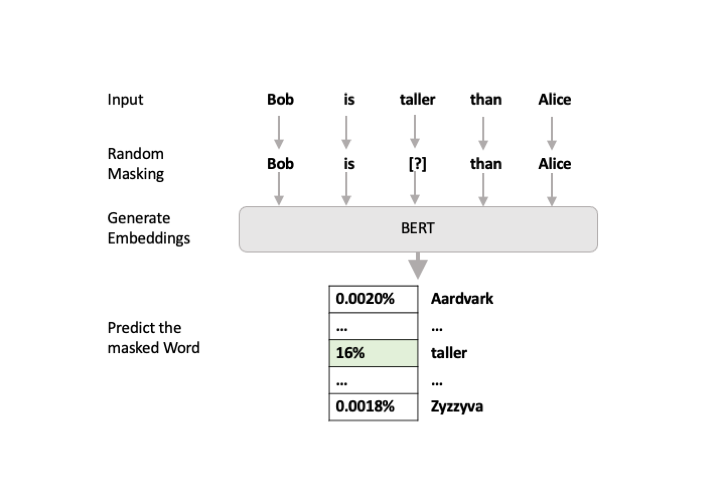
\includegraphics[height=10cm]{ Bilder/preprocessing/BERT/BERT-language-modeling-masked-lm.png}
             	\caption[Training BERT with the MLM task]{Training BERT with the MLM task \cite{alammarIllustratedBERTELMo}}
         		\label{fig:mlm}    
         \end{figure}
            
         
               BERT is trained with millions of Wikipedia articles, meaning the inputs is a large text database. The text segment is split into tokens, which are then encoded as a vector of length 768 \cite[p.~3]{BERT}. Next follows the positional encoding. When applying the transformer encoder to a sequence of words, the output should be dependent of the sequence of the input words. E.g. the sentences "Bob is taller than Alice" and "Alice is taller than Bob" should be encoded as two different vectors. This can be realized with encoding the position of each token. 
               

               
               The token embedding and its positional encoding are now added, and fed into the encoder \cite{illustratedTransformer}. Inside the encoder, four elements process the input sequentially:
               
               \begin{enumerate}
               	\item The self-attention mechanism allows for the model to incorporate the context of a token into its encoding. The mechanism does so by calculating the importance of inputs with themselves ("self") and returns which tokens are important to each other's meaning ("attention").
               	\item To reduce the computational requirements for training a deep neural network, the layers of neurons in the networks are normalized with respect to their activation. This reduced the training time while not impacting the result, which is only dependent on the learning algorithm \cite[p.~10]{baLayerNormalization2016}.
               	\item The \ac{FFNN} takes the results of the layer normalization and the residual connection as input. When the whole transformer is trained on a specific task, the parameters (weights) of this model are also trained. Therefore, the \ac{FFNN} is one gear in the whole process of reaching the transformer's task.
               	\item Finally, the results are normalized again.
               \end{enumerate}
       			
       			 \begin{figure}[h!]
       				\label{fig:encoder}
       				\centering
       				\includegraphics[height=7cm]{Bilder/preprocessing/BERT/encoder.png}
       				\caption[The Transformer Encoder Architecture]{The Transformer Encoder Architecture  \cite{illustratedTransformer}}
       			\end{figure}
			
            
            Evaluating all different models for word vectorization, BERT clearly outperforms the distribustional representations:
            \begin{itemize}
            	\item Word embeddings produce dense and lower-dimensional vectors than distributional representations.
            	\item With word embeddings, the resulting vectors perform a lot better on common \ac{NLP} tasks, meaning the resulting vectors are of higher quality than with distributional representations.
            	\item BERT can process out-of-vocabulary words, this is a big advantage to previous embeddings.
            \end{itemize}

			The advantage of BERT over the other presented options is obvious. But, now there are two unconsidered restrictions:
			First, BERT only encodes words.
			Second, BERT is only in one language.
			
			Luckily, researchers around BERT encountered similar tasks and developed a new BERT model to solve this. 
			First, the Sentence-BERT embeddings are generated in a way that requires only minimal additions to the BERT architecture \cite[p.~2]{sentenceBERT}. Sentence-BERT is trained with a dataset of sentences, labeled with their relationship (contradiction, entailment, neutral) \cite[p.~4]{sentenceBERT}. Two sentences each pass through a BERT model. A pooling layer for each of the two calculates a weighted sum of all words in the sentence to create the embedding for the whole sentences. With the labels and the comparison of two sentence embeddings, the pooling layer is trained. The weights in both pooling layers are adjusted over time, creating a so-called Siamese Network.
			
			Secondly, the embeddings need to be able to understand different languages. A multilingual implementation of BERT can solve this. A multilingual embedding should align vectors in different languages in such a way, that translated sentences are very close in the vector space. A multilingual Sentence-BERT model trains on a dataset with sentences and their translation \cite[p.~2]{mBERT}. The weights in the BERT model are adjusted by completing the task of assigning the same sentence in different languages a similar vector \cite[p.~2]{mBERT}.
			
			Both the multilingual and sentence embeddings require very little additional complexity compared to the underlying BERT model. But, these additions help to accurately represent the content in the dataset.
			
            \subsection{Theoretical Implementation}
            
           	After explaining and evaluating the alternatives, the most favorable one, the word embeddings using \ac{BERT} will be put into practice. In theory, a BERT model would have to be trained using a large text dataset. This took the developers of BERT at Google 4 whole days, and required 4 \ac{TPU}s \cite{BERTTraining}. Fortunately, the researchers published this trained model, making it free to use for the public \cite[p.~2]{BERT}.
            	
            From the available pre-trained models, the \lstinline|distiluse-base-multilingual-cased| model fulfills all the requirements (sentence embeddings, multilingual vector alignment). The prefix 'distiluse' stands for distilled universal sentence encoder, meaning the sentence encoder is compressed in a model with a more portable size. The suffix 'cased' means that words are handled case-sensitive.
            
            Since the description data has already been transformed into a usable format and cleaned, the descriptions can now easily be fed into the \lstinline|distiluse-base-multilingual-cased| model.
            	
            \subsection{Practical Implementation}
             
             The model can be laded using the library \lstinline|sentence_transformers|. The library can create a model from the name of the transformer. Embeddings can be generated very easily, and are returned as a 2D-array. This inference takes about 30ms. For all 79.741 documents, this means an total time of about 40 minutes.
             
\begin{lstlisting}[language=python,
	label=code:generate-embed,
	caption=Generating an Embedding with BERT,
	style=EigenerPythonStyle]   

from sentence_transformers import SentenceTransformer
model = SentenceTransformer(
	'sentence-transformers/distiluse-base-multilingual-cased-v2'
	)
sentence = ["Service Charge for Flight FRA-LAX"]
embedding = model.encode(sentence)
print(embedding)
>>> 	[[-0.02105838 -0.01305696 -0.0403975  ...  0.08315323  0.06774105  0.03354893]
\end{lstlisting}

		Since data cleaning and data wrangling could be sped up significantly with multiprocessing, it stands to reason that this might also work for the inference on BERT. Batching and parallel processing only provides a speed-up if the model can utilize a strong \ac{GPU} \cite{schopfParallelInferenceHuggingFace2022}. This is not the case, so we settle with a one-time processing taking 40 minutes.
		
		During processing, the hardware was overheating and shutting down. To prevent losing progress, batches of 1000 documents were processed at a time, serialized and written on the hard disk. Upon completion, the files are loaded into memory again and unified into one collection of 20MB in vectors.

		These vectors are now ready for clustering.            